\documentclass{article}
\usepackage[utf8]{inputenc}
\usepackage{graphicx}


\title{Reprova Álgebra Linear - Exercícios 2 e 3}
\author{Gabriela Duarte Maciel }
\usepackage{geometry}

\date{29 de outubro de 2022}

\begin{document}

\maketitle





\section{Exercício 2}\label{ex2}
Considere o conjunto S = \{(1, 1, 1, 1, 1),(2, 0, −1, 1, 3),(3, 1, 0, 2, 4),(2, 2, 5, 8, −1),(0, 1, 0, 2, 3)\}.
\begin{itemize}
    \item S é LI ou LD?

\end{itemize}
\mathbf{S = }
\begin{hbox}{

$\left[
\begin{tabular}{ccccc|c}
1 & 2 & 3 & 2 & 0 & 0 \\
1 & 0 & 1 & 2 & 1 & 0 \\
1 & -1 & 0 & 5 & 0 & 0 \\
1 & 1 & 2 & 8 & 2 & 0 \\
1 & 3 & 4 & -1 & 3 & 0

\end{tabular}
\right]

\textbf{l2\leftarrow l2-1*l1}
\\\\
$\left[
\begin{tabular}{ccccc|c}
1 & 2 & 3 & 2 & 0 & 0 \\
0 & -2 & -2 & 0 & 1 & 0 \\
1 & -1 & 0 & 5 & 0 & 0 \\
1 & 1 & 2 & 8 & 2 & 0 \\
1 & 3 & 4 & -1 & 3 & 0


\end{tabular}
\right]
$}
\end{hbox}
\\\\\\\\\\
\xrightarrow{l3\rightarrow l3-1*l1}
\begin{hbox}{

$\left[
\begin{tabular}{ccccc|c}
1 & 2 & 3 & 2 & 0 & 0 \\
0 & -2 & -2 & 0 & 1 & 0 \\
0 & -3 & -3 & 3 & 0 & 0 \\
1 & 1 & 2 & 8 & 2 & 0 \\
1 & 3 & 4 & -1 & 3 & 0
\end{tabular}
\right]

$
$$\xrightarrow{l4\rightarrow l4-1*l1}
\\\\
$\left[
\begin{tabular}{ccccc|c}
1 & 2 & 3 & 2 & 0 & 0 \\
0 & -2 & -2 & 0 & 1 & 0 \\
0 & -3 & -3 & 3 & 0 & 0 \\
0 & -1 & -1 & 6 & 2 & 0 \\
1 & 3 & 4 & -1 & 3 & 0
\end{tabular}
\right]\\
$
\end{hbox}\\
\\\\\\\\\\
\xrightarrow{l5\rightarrow l5-1*l1}
\begin{hbox}{

$\left[
\begin{tabular}{ccccc|c}
1 & 2 & 3 & 2 & 0 & 0 \\
0 & -2 & -2 & 0 & 1 & 0 \\
0 & -3 & -3 & 3 & 0 & 0 \\
0 & -1 & -1 & 6 & 2 & 0 \\
0 & 1 & 1 & -3 & 3 & 0
\end{tabular}
\right]

$
$$\xrightarrow{l3\rightarrow l3-(3/2)*l2}
\\\\
$\left[
\begin{tabular}{ccccc|c}
1 & 2 & 3 & 2 & 0 & 0 \\
0 & -2 & -2 & 0 & 1 & 0 \\
0 & 0 & 0 & 3 & (-3/2) & 0 \\
0 & -1 & -1 & 6 & 2 & 0 \\
0 & 1 & 1 & -3 & 3 & 0
\end{tabular}
\right]\\
$
\end{hbox}\\
\\\\\\\\\\
\xrightarrow{l4\rightarrow l4-(1/2)*l2}
\begin{hbox}{

$\left[
\begin{tabular}{ccccc|c}
1 & 2 & 3 & 2 & 0 & 0 \\
0 & -2 & -2 & 0 & 1 & 0 \\
0 & 0 & 0 & 3 & (-3/2) & 0 \\
0 & 0 & 0 & 6 & (-3/2) & 0 \\
0 & 1 & 1 & -3 & 3 & 0
\end{tabular}
\right]

$
$$\xrightarrow{l5\rightarrow l5-(-1/2)*l2}
\\\\
$\left[
\begin{tabular}{ccccc|c}
1 & 2 & 3 & 2 & 0 & 0 \\
0 & -2 & -2 & 0 & 1 & 0 \\
0 & 0 & 0 & 3 & (-3/2) & 0 \\
0 & 0 & 0 & 6 & (3/2) & 0 \\
0 & 0 & 0 & -3 & (7/2) & 0
\end{tabular}
\right]\\
$
\end{hbox}\\
\\\\\\\\\\
\xrightarrow{l4\rightarrow l4-2*l3}
\begin{hbox}{

$\left[
\begin{tabular}{ccccc|c}
1 & 2 & 3 & 2 & 0 & 0 \\
0 & -2 & -2 & 0 & 1 & 0 \\
0 & 0 & 0 & 3 & (-3/2) & 0 \\
0 & 0 & 0 & 0 & (9/2) & 0 \\
0 & 0 & 0 & -3 & (7/2) & 0
\end{tabular}
\right]

$
$$\xrightarrow{l5\rightarrow l5-(-1)*l3}
\\\\
$\left[
\begin{tabular}{ccccc|c}
1 & 2 & 3 & 2 & 0 & 0 \\
0 & -2 & -2 & 0 & 1 & 0 \\
0 & 0 & 0 & 3 & (-3/2) & 0 \\
0 & 0 & 0 & 0 & (9/2) & 0 \\
0 & 0 & 0 & 0 & 2 & 0

\end{tabular}
\right]\\
$
\end{hbox}\\
\\\\\\\\\\
\xrightarrow{l5\rightarrow l5-(-4/9)*l4}
\begin{hbox}{

$\left[
\begin{tabular}{ccccc|c}
1 & 2 & 3 & 2 & 0 & 0 \\
0 & -2 & -2 & 0 & 1 & 0 \\
0 & 0 & 0 & 3 & (-3/2) & 0 \\
0 & 0 & 0 & 0 & (9/2) & 0 \\
0 & 0 & 0 & 0 & 0 & 0
\end{tabular}
\right]\\
$
\end{hbox}\\
\\\textit{R: Portanto, é LD}\\\\
\begin{itemize}
   \item Forma base do R-espaço vetorial R5?
   \\\textit{R:Como S é ld, ele não forma uma base de R^5}
\end{itemize}












































































    
\end{hbox}
\newpage
\section{Exercício 3}\label{ex3}
 Considere o conjunto W = \{(x, y, z, w, t, u) \mid  x, y, z, w, t, u \in R \land x + y + w + z + t + u = 0 \land y -  w - z = 0 \land w + t - x = 0\} \subseteq R^6. 


\item Mostre que conjunto W é um subespaço do R-espaço vetorial R^6 .

\\t – x = 0 

t = x 

y – w – z = 0 

y = w + z 

x + y + w + z + t + u = 0 \to  x + w + z + w + z + x + u = 0 

u = -x -y -w -z -t \to u = -2x -2w -2z 

W = \{(x, w + z, z, w, x, - x – w – z – w – z – x)\} \to

W = \{(x, w + z, z, w, x, - 2x – 2w – 2z)\mid x, z, w \in R\}\\

I) 0 \in W para x = 0 z = 0 w = 0 

(w, w, w, w, w, -w) \to (x, w + z, z, w, x, - 2x – 2w – 2z) 

= (0, 0, 0, 0, 0, -0) 

= 0 

Logo, 0 \in W\\ 

II) u, z \in W \to  u + z \in W, sendo:  

u = (u1, u2, u3, u4, u5, -u6) \to (x_1, w_1 + z_1, z_1, w_1, x_1, - 2x_1 – 2w_1 – 2z_1) 

z = (z1, z2, z3, z4, z5, -z6) \to (x_2, w_2 + z_2, z_2, w_2, x_2, - 2x_2 – 2w_2 – 2z_2)  

u + z = (x_1 + x_2, (w_1+z_1) + (w_2+z2) , z_1 + z_2, w_1 + w_2, x_1 + x_2, (-2x_1 -2w_1 - 2z_2) + (-2x_2 - 2w_2 - 2z_2)) 

u + z= (x_1 + x_2, w_1+z_1+w_2+z_2, z_1+z_2, w_1+w_2, x_1+x_2, -2x_1-2x_2,-2w_1-2w_2,-2z_1-2z_2) 

Logo, u + z \in W \\

III) a \in R, v \in W \to av \in W, sendo:  

v = (v1, v2, v3, v4, v5, -v6) \to (x, w + z, z, w, x, - 2x – 2w – 2z) 

av = a . (x_1, w_1+z_1, z_1, w_1, x_1, -2x_1-2w_1-2z_1) 

 av = (a. x_1, a . w_1+z_1, a . z_1, a . w_1, a . x_1, a. -2x_1-2w_1-2z_1)  

av = (ax_1, aw_1w_2, az_1, aw_1, ax_1, a-2x_1-2w_1-2z_1) 

Logo, av \in W. \\

Logo W é subespaço vetorial de R6.\\

\begin{itemize}
\\\item O conjunto W = \{(x, y, z) \mid  x, y, z \in R \land x - z = 1 \land  y + x = 0\} \end{itemize}
    
    \item é um subsespaço vetorial de R3? Esboce graficamente W.\\

x – z = 1 \to x = 1 + z

y + x = 0 \to y + 1 + z = 0 \to y = -1 – z. 

W = \{(1 + z, -1 - z, z)\} \\

I) 0 \in W, para z = 0 

(1 + z, - 1 – z, z) \to (1 + 0, - 1 – 0, 0) = (1, -1, 0).  

Logo 0 NÃO pertence a W para z = 0. Portanto, W NÃO é subespaço vetorial.\\ 

\begin{figure}[!h]
\centering
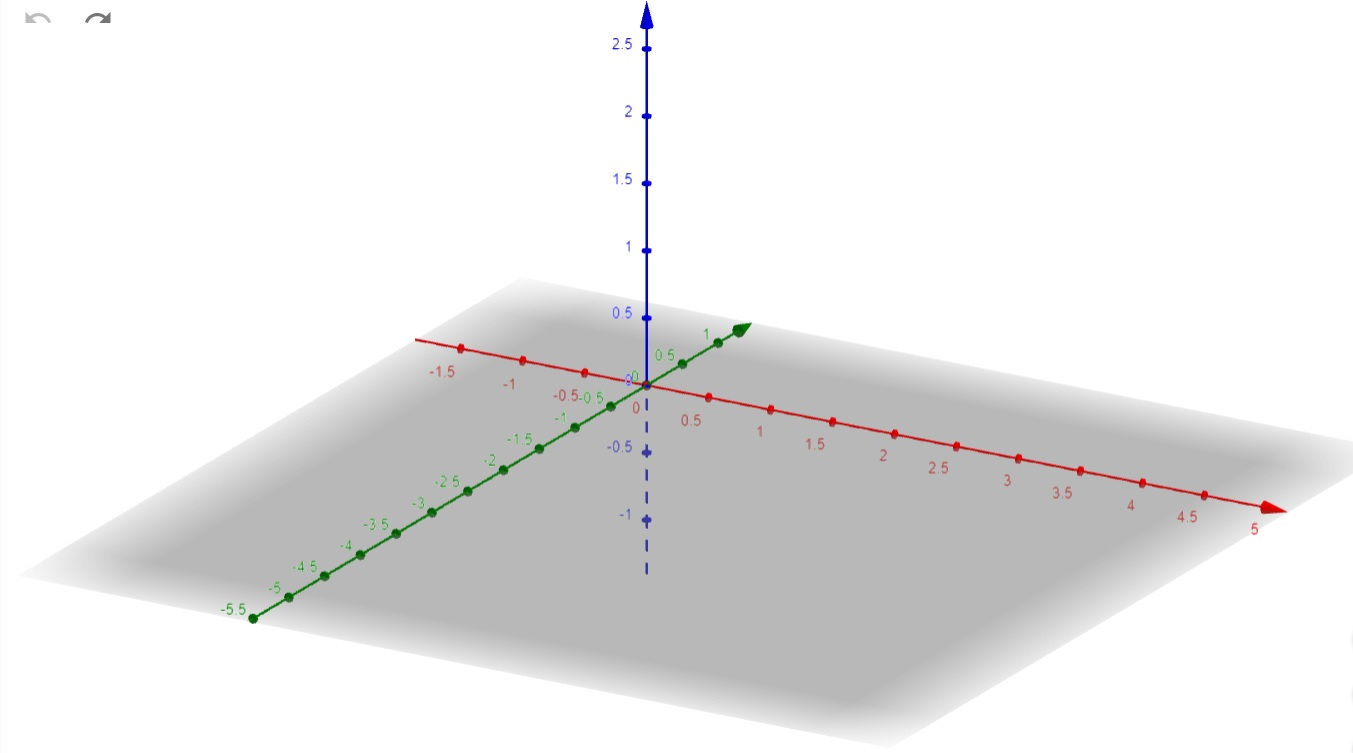
\includegraphics[width=10cm]{graficoquestao3.jpg}
\caption{Representação gráfica.}
\label{fig:graficoquesto3.jpg}
\end{figure}


\begin{itemize}

\item Invente seu subespaço vetorial em qualquer R n com n maior igual a 2. Mostre que o conjunto apresentado é de fato
um subespaço vetorial. Não vale usar nenhum exemplo da aula ou da prova
\end{itemize}

W = \{(x, y, z) \mid  x + y -2z = 0 \} 

 

x + y -2z = 0

x = -y + 2z 

 
W= {(-y + 2z, y, z) \mid y,z \in R\}\\


 

I) (0,0,0) \in W, pois: y,z = 0 \\




II) v, w, x \in W \to  v + w + x \in W, sendo:  

v = (-y1 + 2z1, y1, z1)

w = (-y2 + 2z2, y2, z2)

z = (-y3 + 2z3, y3, z3)

v + w + z  = (-y1 + 2z, y1, -2y1) + (-y2 + 2z2, y2, z2) + (-y3 + 2z3, y3, z3)

u + w + z = (-y1+2z1-y2+2z2-y3+2z3,y1+y2+y3,-2y1+z2+z3) 

Logo, u + w + z \in W\\

III) a \in R, v \in Z \to av \in W. Sendo:  

v = (v1,v2,v3)  \to (-y1 + 2z1, y1, z1)  

a.v = a . (-y1 + 2z1, y1, z1) 

a.v = (a . (-y1 +2z1), a . y1, a . z1) 

a.v = (-ay1 + a2z1, ay1, -az1) 

Logo, av \in W \\

Logo W é subespaço vetorial de R3 \\

\end{itemize}
\end{document}
